\pgfplotsset{compat=1.18}

\chapter{Momentum and Impulse}

The first section of this class typically covers momentum, impulse, and 
conservation of momentum.  For reference, these three ideas are given below
in mathematical form.

\begin{align}
    \vect{p} &= m\vect{v} \tag{Momentum} \\
    \vect{J} &= \Delta \vect{p} = \vect{F}_{\text{avg}}\Delta t \tag{Impulse} \\
    \sum \vect{p}_{\text{initial}} &= \sum \vect{p}_{\text{final}} \tag{Conservation of Momentum}
\end{align}


\textbf{All} problems in this section can be solved only with the above equations! 
Take careful note that the conservation of momentum condition is a \textit{vector} sum! Also take note
of the impulse equation used here. This form is only valid for a constant force.  Calculus 1
is a co-requisite for this course, so at this point student will likely not be familiar
or comfortable with the idea of an integral.\\

In addition to these equations, you will also need to know how to break vectors into components, 
since we will be dealing with some two-dimensional problems. The most important picture
for knowing how to accomplish this is shown below. \\

\vspace{2em}

\begin{center}
    \begin{tikzpicture}
        \draw[->, >=Stealth, thick] (0,0) -- (4,3) node[midway, above] {$\vect{A}$};
        \draw[->, >=Stealth, thick] (0,0) -- (4,0) node[midway, below] {$A_x = A \cos \theta$};
        \draw[->, >=Stealth, thick] (4,0) -- (4,3) node[midway, right] {$A_y = A \sin \theta$};
        \draw (4,0) -- (4,3) -- (0,0);
        \node at (.7, 0.25) {$\theta$};
        \draw (0.3,0) arc (0:36.87:0.3);
        \node at (2,-2) {Right Triangle Representation of Vector};
        % Draw arc and label phi in the upper right corner
        \draw (4,2.6) arc (-90:-160:0.3);
        \node at (3.75,2.4) {$\phi$};
        \node at (2.3,-0.75) {$=A \sin \phi$};
        \node at (5.5,1) {$=A \cos \phi$};
    \end{tikzpicture}
\end{center}

If you are teaching this course, you will be explaing this diagram \textbf{very} frequently.
Make sure you understand it well, and can explain it clearly to students! We have included a
large format version of this same picture on the first page for easy reference. Trust us, you'll need it. \\ 

\newpage
\section{Momentum Tutorial 1: Oomph}

\textbf{Approximate Time:} 50 minutes \\
\textbf{Equipment Needed:} None \\
\textbf{Pre-Lecture Required?}: No \\

This introductory tutorial is meant to do two things: (1) introduce students to the idea of momentum
and impulse, and (2) get students used to studio mode and working in groups (assuming this is
the first assignment of the semester). \\

The tutorial introduces the concept of momentum under the guise of \textbf{``oomph''} (a non-technical term
for momentum). The students are asked to make qualitative predictions about the oomph of various objects
of different masses and speeds.  Ideally, the students will come to the conclusion that oomph is proportional
to both mass and speed, and that the mathematical expression for oomph is $p = mv$.\\

The second section of the tutorial introduces the idea of impulse, and how a force acting over a time interval
can change an object's momentum.  The students are asked to make qualitative predictions about how the
change in momentum depends on the force applied to an object and how long it is applied for.  Ideally, the students will come to the conclusion
that the change in oomph is proportional to both the force and the time interval, and that the mathematical expression for impulse is
$J = F \Delta t$. \\

At this stage, it is enough that students understand what these two concepts are.  You will note
that none of the equations are written in vector form.  This is intentional, as we will introduce
the vector nature of momentum and impulse in the next tutorial.  For now, we want students
to get comfortable with the concepts in one dimension. \\

\begin{tutorialbox}[title=Student Issue 1: Forces over Time]
A common issue that students have is believing that applying a force
over 5 seconds and applying the same force over 10 seconds both result in the same 
momentum in the end.  It is often because students operate under a sort of "maximum" 
force idea, where they are thinking about \textit{themselves} pushing the object.
Since a person has a maximum force they can apply (and because friction and other things
exist), in reality you can really only speed things you're pushing up to a certain point, 
so time doesn't seem to matter. A good example to use in these cases are rocket ships in space.
\end{tutorialbox}

\begin{problembox}[title=Learning Outcomes: Oomph]
\begin{enumerate}[label=(\alph*)]
    \item Momentum is a measure of mass in motion and is calculated by $p = mv$.
    \item Impulse is a measure of an object's \textbf{change} in momentum, and is calculated by \\ $J = F \Delta t = \Delta p$.
    \item Group work and discussions should be written out clearly on whiteboards.
\end{enumerate}
\end{problembox}

\newpage
\section{Momentum Problem Set 1: Impulse in One Dimension}
\textbf{Approximate Time:} 50 minutes \\
\textbf{Equipment Needed:} None \\
\textbf{Pre-Lecture Required?}: Yes - Area under the curve integration\\

Each of these problems can be solved by first finding the impulse, either by using
$J = F \Delta t$ for constant forces, or by finding the area under the curve for variable forces, 
in which cases a graph is provided.\\


\noindent
\textbf{Problem 1:} A 50.0 kg archer, standing on frictionless ice, shoots a 100.0 g 
arrow at a speed of 100.0 m/s. The direction that the arrow travels is defined to 
be the positive direction.
\begin{enumerate}[label=(\alph*)]
    \item What is the sign of the impulse (positive or negative)imparted to the arrow?
    \item What magnitude impulse did the archer impart to the arrow?
    \item Estimate (just make a guess, .1 s, .5 s, 2 s, etc.) how much time the string on the bow was in contact with the arrow.
    \item Calculate the force the bow string imparted on the arrow.
\end{enumerate}

\begin{tutorialbox}[title = Student Issue: Guessing Values]
You'd be surprised how often students don't realize that making an educated guess 
about how long the bowstring is in contact with the arrow is a perfectly acceptable
thing to do.  If students are struggling with this, remind them that they are not being
asked to calculate the exact force, just to estimate it.
\end{tutorialbox}

\newpage
\noindent
\textbf{Problem 2:}  A miniature sled with a mass of 8.0 kg is sliding across the 
ice to the right with a speed of 2.0 m/s when it hits a rough patch in the ice. 
The force of friction for this rough patch of ice is shown as a function of time 
in the figure below. To the right is defined to be positive direction.

\begin{enumerate}[label=(\alph*)]
    \item How will the sled’s speed change during the rough patch? 
    Explain how your intuitive answer compares to the information given in the graph.
    \item Calculate the sled’s speed and direction after the rough patch. 
    Explain how this answer compares to your intuition.
\end{enumerate}
    
\begin{center}
    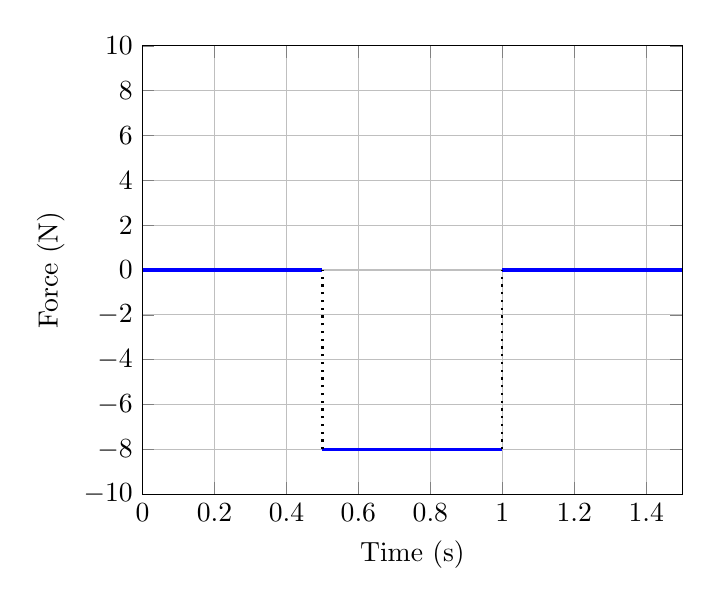
\begin{tikzpicture}
        \begin{axis}[
            xlabel={Time (s)},
            ylabel={Force (N)},
            ymin=-10, ymax=10,
            xmin=0, xmax=1.5,
            grid=major,
            ytick={-10,-8,...,10}
        ]
        \addplot[blue,very thick,domain=0:0.5, samples=2] {0};
        \addplot[blue,very thick,domain=0.5:1, samples=2] {-8};
        \addplot[blue,very thick,domain=1:1.5, samples=2] {0};
        % Dotted vertical lines at discontinuities
        \addplot[dotted, thick, black, domain=-10:10] coordinates {(0.5,-8) (0.5,0)};
        \addplot[dotted, thick, black, domain=-10:10] coordinates {(1,-8) (1,0)};
    \end{axis}
    \end{tikzpicture}
\end{center}

\begin{tutorialbox}[title = Student Issue: Negative Area]
Take note that the area under the curve here is negative, since the force is negative. 
While students typically do in fact correctly state that the impulse is negative here, it often
comes purely from a physical intuition standpoint (friction slows things down), and they don't actually calculate the area numerically,
with the negative 8 Newton force.
\end{tutorialbox}
\begin{tutorialbox}[title = Student Issue: Step Functions]
    A handful of students will argue about the nature of the force graph here.  They will say that
    the force can't just instantaneously jump from 0 to -8 N, and then back to 0 N.  Try to keep
    them on the critical moments here, not the transition points. Assure them that this graph is an
    \textbf{idealized} representation to help focus on the key concepts.
\end{tutorialbox}

\newpage

\noindent
\textbf{Problem 3:} Far in space, where gravity is negligible, a 425 kg rocket traveling 
at 75 m/s fires its engines. The figure shows the thrust force as a function of time. 
The mass lost by the rocket during these 30.0 s is negligible. Up is defined to be the 
positive direction.

\begin{enumerate}[label=(\alph*)]
    \item Describe how the rocket's speed changes in the time intervals (i) 0-10 s and (ii) 10-30 s.
    \item Calculate the rocket's speed at 10 s and at 30 s.
    \item Are your answers to (a) and (b) consistent? If not, explain how you would change your answers to make them consistent.
\end{enumerate}

\begin{center}
    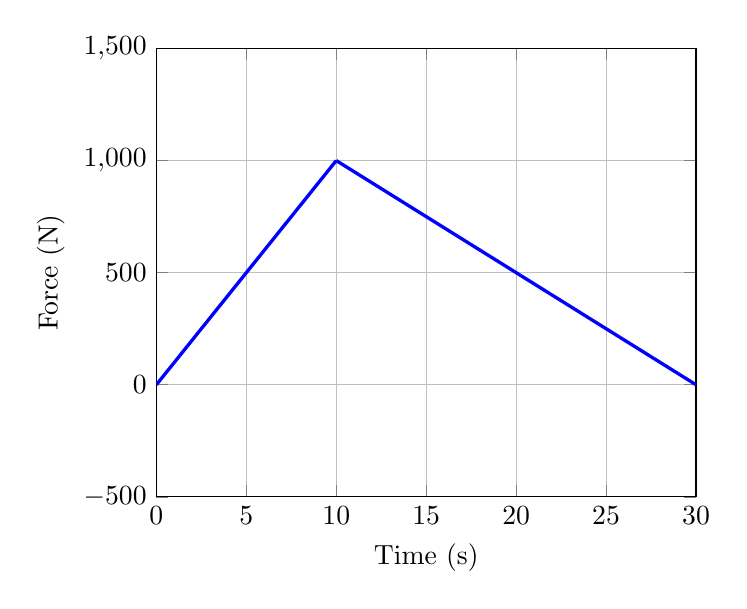
\begin{tikzpicture}
        \begin{axis}[
            xlabel={Time (s)},
            ylabel={Force (N)},
            ymin=-500, ymax=1500,
            xmin=0, xmax=30,
            grid=major,
            ytick={-500,0,500,1000,1500}
        ]
        \addplot[blue,very thick,domain=0:10, samples=2] {100*x};
        \addplot[blue,very thick,domain=10:30, samples=2] {-50*x + 1500};
    \end{axis}
    \end{tikzpicture}
\end{center}

\begin{tutorialbox}[title = Student Issue: Negative Slope $\neq$ Slowing Down]
    A very common mistake made on this problem is that during the first 10 seconds, the rocket 
    is speeding up, which is true.  However, students will then go on to say that the rocket is
    slowing down during the next 20 seconds, which is not true.  The force here is \textbf{always}
    positive, meaning the rocket is always speeding up.  The force is just not as large during
    the second time interval, so the rocket is still speeding up, just not as quickly.
\end{tutorialbox}

\vspace{2em}

\noindent
\textbf{Problem 4:} A monkey throws a lime.  The lime has a mass of 0.3 kg and it is 
thrown at an initial velocity of 80 m/s (this particular monkey has realized there are 
no limits to monkey strength). The lime flies across the jungle until it hits MonkeyMan 
Steve in the face.  It is in contact with his face for 0.5 s.  What is the force felt 
(in Newtons) by poor poor MonkeyMan Steve?

\begin{problembox}[title=Learning Outcomes: Impulse in One Dimension]
\begin{enumerate}[label=(\alph*)]
    \item Calculate impulse from a force vs. time graph.
    \item Calculate final velocity from impulse and initial velocity.
    \item Understand that a negative force results in a negative impulse.
    \item Solve problems algebraically and numerically.
\end{enumerate}
\end{problembox}